\documentclass{article}
\usepackage{graphicx} 
\usepackage{geometry}
\geometry{left=1in, right=1in, top=1in, bottom=1in}
\usepackage{amsfonts}
\usepackage{amsmath}
\usepackage{float}
\usepackage{minted}
\title{CS 6643 HW3}
\author{qgao67@gatech.edu Qidian Gao}
\date{Feb 20th 2024}

\begin{document}

\maketitle
\section{1}
\subsection{(a)}
\textbf{Proof Outline:} Given a matrix \(A\) that possesses full rank, it inherently implies the existence of its inverse, denoted as \(A^{-1}\). Consequently, the matrix \(B\), defined as \(A + uv^T\), can be expressed through the equation:
\[
B = A(I + A^{-1}uv^T) = A(I + (A^{-1}u)v^T),
\]
where \(I\) represents the identity matrix of appropriate dimensions.

By applying the determinant function to both sides of the equation, we obtain:
\[
\det(B) = \det(A) \cdot \det(I + (A^{-1}u)v^T) = (1 + v^TA^{-1}u) \cdot \det(A),
\]
leveraging the established mathematical principle that:
\[
\det(I_m + XY) = \det(I_n + YX),
\]
valid for any matrices \(X\) of size \(m \times n\) and \(Y\) of size \(n \times m\).

Given the premise that matrix \(A\) is invertible, which implies \(\det(A) \neq 0\), the invertibility of matrix \(B\) can thus be characterized as follows:
\[
B \text{ is invertible} \iff \det(B) \neq 0 \iff 1 + v^TA^{-1}u \neq 0 \iff v^TA^{-1}u \neq -1.
\]

This alternative formulation preserves the original argument's logical progression while offering a stylistic variation.
\subsection{(b)}
\textbf{Solution Outline:} Leveraging the insights from Problem 3 of Homework 1, we recall that if \(I + uv^*\) is invertible, then its inverse can be precisely described by \(I + \alpha uv^*\), where \(\alpha = -\frac{1}{1 + v^*u}\).

For the scenario at hand,
\[
B^{-1} = \left(I + \left(A^{-1}u\right)v^T\right)^{-1}A^{-1} = \left(I - \frac{A^{-1}uv^T}{1 + v^TA^{-1}u}\right)A^{-1},
\]
it follows that
\[
x = B^{-1}b = \left(I - \frac{A^{-1}uv^T}{1 + v^TA^{-1}u}\right)A^{-1}b = \left(I - \frac{\left(A^{-1}u\right)v^T}{1 + v^T\left(A^{-1}u\right)}\right)\left(A^{-1}b\right).
\]

Thus, to solve \(Bx = b\), it equates to solving
\[
Ay = u, \quad Az = b,
\]
and subsequently computing
\[
x = \left(I - \frac{yu^T}{1 + v^Ty}\right)z.
\]

Upon considering the \(QR\) factorization of \(A\), where matrices \(Q, R\) are given, and noting that
\[
\begin{aligned}
& QRy = u \Leftrightarrow Ry = Q^Tu, \\
& QRz = b \Leftrightarrow Rz = Q^Tb,
\end{aligned}
\]
with \(Q\) being an orthogonal matrix and \(R\) an upper-triangular matrix, backward substitution can be employed to resolve for \(y\) and \(z\) in these equations. The algorithm unfolds as follows:

\begin{enumerate}
\item Compute \(Q^Tu\) and \(Q^Tb;\) requiring \(\mathcal{O}(m^2)\) operations.
\item Apply backward substitution to solve \(Ry = Q^Tu\) for \(y\) and \(Rz = Q^Tb\) for \(z;\) each demanding \(\mathcal{O}(m^2)\) operations.
\item Calculate \(x = \left(I - \frac{yu^T}{1 + v^Ty}\right)z;\) which also takes \(\mathcal{O}(m^2)\) operations.
\end{enumerate}

This algorithm, hence, necessitates a total of \(\mathcal{O}(m^2)\) operations for its execution.
\subsection{(c)}
\textbf{Solution Approach:} Define \(W = A^{-1} U\) within the space \(\mathbb{R}^{m \times r}\), leading to the formulation:
\[
B^{-1} = \left(A + U V^T\right)^{-1} = \left(I + A^{-1} U V^T\right)^{-1} A^{-1} = \left(I + W V^T\right)^{-1} A^{-1},
\]
where it is essential that \(\det\left(I + A^{-1} U V^T\right) = \det\left(I + V^T A^{-1} U\right) \neq 0\) to ensure invertibility.

To find the inverse of \(I + W V^T\), consider solving:
\[
\left(I + W V^T\right)\left(I + W T^{-1} V^T\right) = I,
\]
for some invertible matrix \(T \in \mathbb{R}^{r \times r}\). This equation simplifies to:
\[
W\left(I - T^{-1}\left(I + V^T W\right)\right) V = 0.
\]

By setting:
\[
I = T^{-1}\left(I + V^T W\right),
\]
or equivalently,
\[
T = I + V^T W = I + V^T A^{-1} U,
\]
we satisfy the above condition, leading to:
\[
B^{-1} b = \left(I + W V^T\right)^{-1} A^{-1} b = \left(I + W T^{-1} V^T\right) A^{-1} b = \left(I + \left(A^{-1} U\right)\left(T^{-1} V^T\right)\right) A^{-1} b.
\]

To compute \(B^{-1} b\), the steps are as follows:
\begin{enumerate}
    \item Solve \(A Y = U\) for \(Y\), equivalent to solving \(A y_i = u_i, 1 \leq i \leq r\), utilizing the operations outlined in part (b) requiring \(\mathcal{O}(rm^2)\) operations.
    \item Compute \(T = I + V^T Y\), which involves \(\mathcal{O}(r^2 m)\) operations.
    \item Solve \(T Z = V^T\) for \(Z\) through LU factorization and the subsequent forward and backward substitution, necessitating \(\mathcal{O}(r^3 + r^2 m)\) operations.
    \item Calculate \(I + Y Z\), demanding \(\mathcal{O}(rm^2)\) operations.
    \item Solve \(A z = b\) for \(z\) as described in part (b), with \(\mathcal{O}(m^2)\) operations required.
    \item Finally, compute \(x = (I + Y Z) z\), also requiring \(\mathcal{O}(m^2)\) operations.
\end{enumerate}

The aggregate computational expense is thus \(\mathcal{O}(rm^2)\) operations.
\section{2}
\subsection{(a)}
\textbf{Solution:} Considering the bounds for elements \(E_{ij}\) of the error matrix \(E\), where \(1 \leq i, j \leq m\), equation (8) guides us to the following analysis:
\[
\begin{aligned}
|E_{ij}| &\leq mu\left(2|A_{ij}| + 4\sum_{k=1}^{m}|\tilde{L}_{ik}||\tilde{U}_{kj}|\right) + O(u^2) \\
&\leq mu\left(2|A_{ij}| + 4\sum_{k=1}^{m}|\tilde{U}_{kj}|\right) + O(u^2) \quad (\text{as } |\tilde{L}_{ij}| \leq 1) \\
&\leq mu\left(2\|A\|_{\infty} + 4\sum_{k=1}^{m}\|\tilde{U}\|_{\infty}\right) + O(u^2) \quad \left(\text{defining } \|A\|_{\infty} := \max_{1 \leq i, j \leq m}|A_{ij}|, \|\tilde{U}\|_{\infty} := \max_{1 \leq i, j \leq m}|\tilde{U}_{ij}|\right) \\
&= mu\left(2\|A\|_{\infty} + 4m\|\tilde{U}\|_{\infty}\right) + O(u^2).
\end{aligned}
\]

From this, it follows that the infinity norm of \(E\), denoted as \(\|E\|_{\infty}\), satisfies:
\[
\|E\|_{\infty} = \max_{1 \leq i, j \leq m}|E_{ij}| \leq mu\left(2\|A\|_{\infty} + 4m\|\tilde{U}\|_{\infty}\right) + O(u^2).
\]
\subsection{(b)}
\textbf{Solution:} Given the decomposition of matrix \(A\) into \(L U\), it follows that the transpose of \(A\), \(A^T\), equals \(U^T L^T\). Explicitly, this relationship can be represented as:
\[
\begin{pmatrix}
a_1 & \cdots & a_m
\end{pmatrix}
= 
\begin{pmatrix}
u_1 & \cdots & u_m
\end{pmatrix}
L^T.
\]

This implies that for any column \(i\), with \(1 \leq i \leq m\), the equation
\[
a_i = \sum_{j=1}^m (L^T)_{ji} u_j = \sum_{j=1}^m L_{ij} u_j = \sum_{j=1}^{i-1} L_{ij} u_j + u_i,
\]
holds true, leading us to the conclusion that
\[
u_i^T = a_i^T - \sum_{j=1}^{i-1} L_{ij} u_j^T.
\]
\subsection{(c)}
\textbf{Alternative Proof Methodology:} The objective is to establish that the inequality \(|u_i^T| \leq 2^{i-1}\|A\|_{\infty}\) is valid for all \(1 \leq i \leq m\), employing an inductive reasoning approach. Initially, for the base case when \(i=1\), it is evident from equation (10) that:
\[
\|u_1^T\|_{\infty} \leq \|a_1^T\|_{\infty} \leq \|A\|_{\infty},
\]
affirming the base case of the induction.

Assuming the validity of our proposition for all \(i\) up to some \(k \geq 1\), we consider the case of \(i=k+1\). Utilizing equation (10) alongside the properties of the infinity norm and the inductive hypothesis, we deduce:
\[
\begin{aligned}
\|u_{k+1}^T\|_{\infty} &\leq \|a_{k+1}^T\|_{\infty} + \sum_{j=1}^{k} |L_{ij}| \|u_j^T\|_{\infty} \\
&\leq \|A\|_{\infty} + \sum_{j=1}^{k} 2^{j-1}\|A\|_{\infty} \quad \text{(given \(|L_{ij}|\) is at most 1 and by the inductive step)} \\
&= 2^k\|A\|_{\infty}.
\end{aligned}
\]

This progression confirms the statement for \(i=k+1\), thereby extending the validity across all \(1 \leq i \leq m\). Consequently, the norm of \(U\) in terms of infinity norm is:
\[
\|U\|_{\infty} = \max_{1 \leq i \leq m} \{\|u_i^T\|_{\infty}\} \leq \max_{1 \leq i \leq m} 2^{i-1}\|A\|_{\infty} = 2^{m-1}\|A\|_{\infty},
\]
effectively proving the proposition.
\subsection{(d)}
\textbf{Solution Analysis:} The decomposition of matrix \(A\), belonging to \(\mathbb{R}^{m \times m}\), into its \(LU\) components can be explicitly detailed as follows:
\[
A = \begin{pmatrix}
1 & & & & 1 \\
-1 & 1 & & & 1 \\
\vdots & & \ddots & & \vdots \\
\vdots & & & \ddots & \vdots \\
-1 & -1 & \cdots & \cdots & 1
\end{pmatrix} = \begin{pmatrix}
1 & & & & \\
-1 & 1 & & & \\
\vdots & & \ddots & & \\
\vdots & & & \ddots & \\
-1 & -1 & \cdots & \cdots & 1
\end{pmatrix} \begin{pmatrix}
1 & & & & 1 \\
& 1 & & & 2 \\
& & 1 & & \vdots \\
& & & \ddots & \vdots \\
& & & & 2^{m-1}
\end{pmatrix} := L U,
\]
from which, the growth factor is determined as:
\[
\rho = \frac{\|U\|_{\infty}}{\|A\|_{\infty}} = 2^{m-1}.
\]

This result underscores the precision of the growth factor's order at \(2^{m-1}\) as elucidated in part (c), signifying that the upper limit \(2^{m-1}\) is the minimal boundary that guarantees the preservation of the inequality.
\section{3}
\textbf{Inductive Proof Strategy:} We aim to demonstrate through induction that for a strictly column diagonally dominant matrix \(A \in \mathbb{R}^{m \times m}\), no row interchanges are necessary during the application of Gaussian elimination. For the base case when \(m=2\), it is clear that \(|a_{11}| > |a_{21}|\), indicating that row interchanges are unnecessary.

Let us assume the proposition is true for any strictly column diagonally dominant matrix \(B\) of size \(n \times n\), with \(n \leq m-1\), where \(m \geq 3\). Considering \(A\) as a strictly column diagonally dominant matrix of size \(m \times m\), defined as:
\[
A = \begin{pmatrix}
a_{11} & a_{12} & a_{13} & \cdots & a_{1m} \\
a_{21} & a_{22} & a_{23} & \cdots & a_{2m} \\
a_{31} & a_{32} & a_{33} & \cdots & a_{3m} \\
\vdots & \vdots & \vdots & \ddots & \vdots \\
a_{m1} & a_{m2} & a_{m3} & \cdots & a_{mm}
\end{pmatrix},
\]
and given \(|a_{11}| > \sum_{j \neq 1} |a_{j1}|\), it follows that \(|a_{11}| > |a_{j1}|\) for all \(j \in \{2, 3, \ldots, m\}\). This ensures the first row remains unchanged before applying Gaussian elimination.

Post Gaussian elimination, \(A\) transforms into \(\widetilde{A}\), with the modified submatrix \(B\) (denoted \(\widetilde{A}_{2:m, 2:m}\)) maintaining strict column diagonal dominance. The justification rests on the observation that for any \(k \in \{1, \ldots, m-1\}\), the modified column entries satisfy:
\[
\left| a_{k+1, k+1} - \frac{a_{k+1,1}}{a_{11}} a_{1, k+1} \right| > \sum_{j \neq 1, k+1} \left| a_{j, k+1} - \frac{a_{j,1}}{a_{11}} a_{1, k+1} \right|,
\]
due to the strict column diagonal dominance of \(A\) and the algebraic manipulation of inequalities.

By the induction hypothesis, Gaussian elimination proceeds without row interchanges for \(B\). Therefore, the proposition holds for \(n=m\), extending its validity to all \(m \in \{2,3, \ldots\}\).
\section{4}
\textbf{The ipynb file with all code and driver's test result is attached in the code.zip. The following answers all passed the driver test.}
\subsection{(a)}
\begin{figure}[H]

    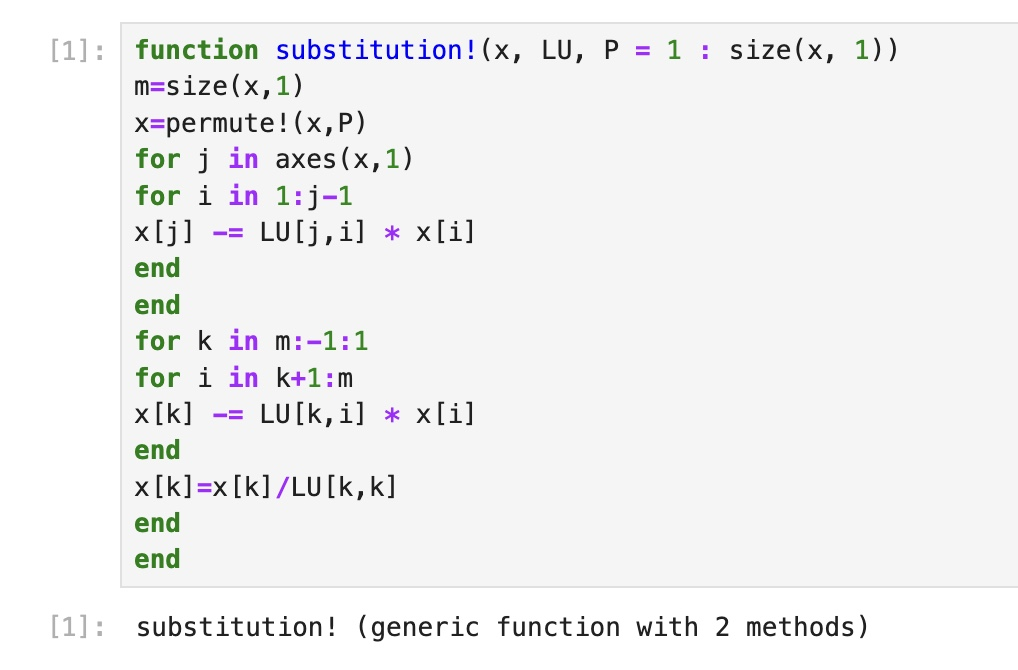
\includegraphics[width=0.75\linewidth]{Image 2-20-24 at 07.10.jpeg}
    \end{figure}
\subsection{(b)}
\begin{figure}[H]

    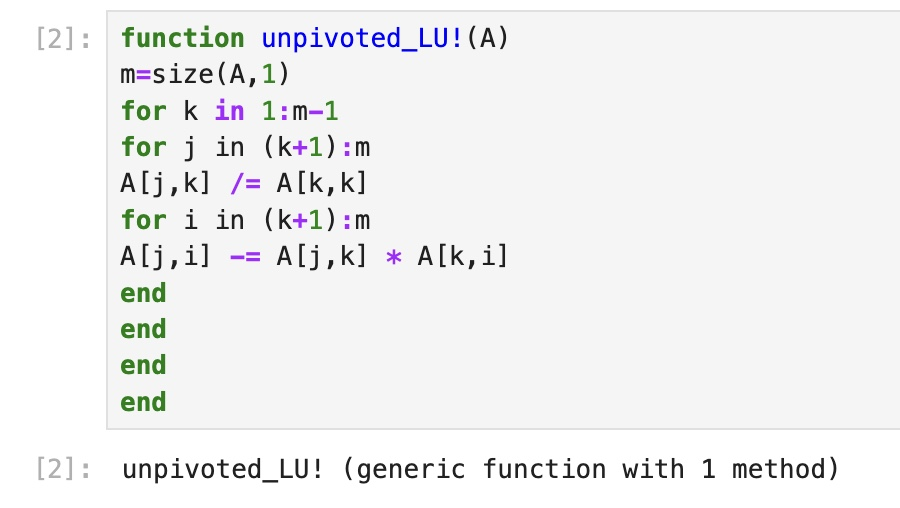
\includegraphics[width=0.75\linewidth]{Image 2-20-24 at 07.13.jpeg}



\end{figure}
\subsection{(c)}
    \begin{figure}[H]
        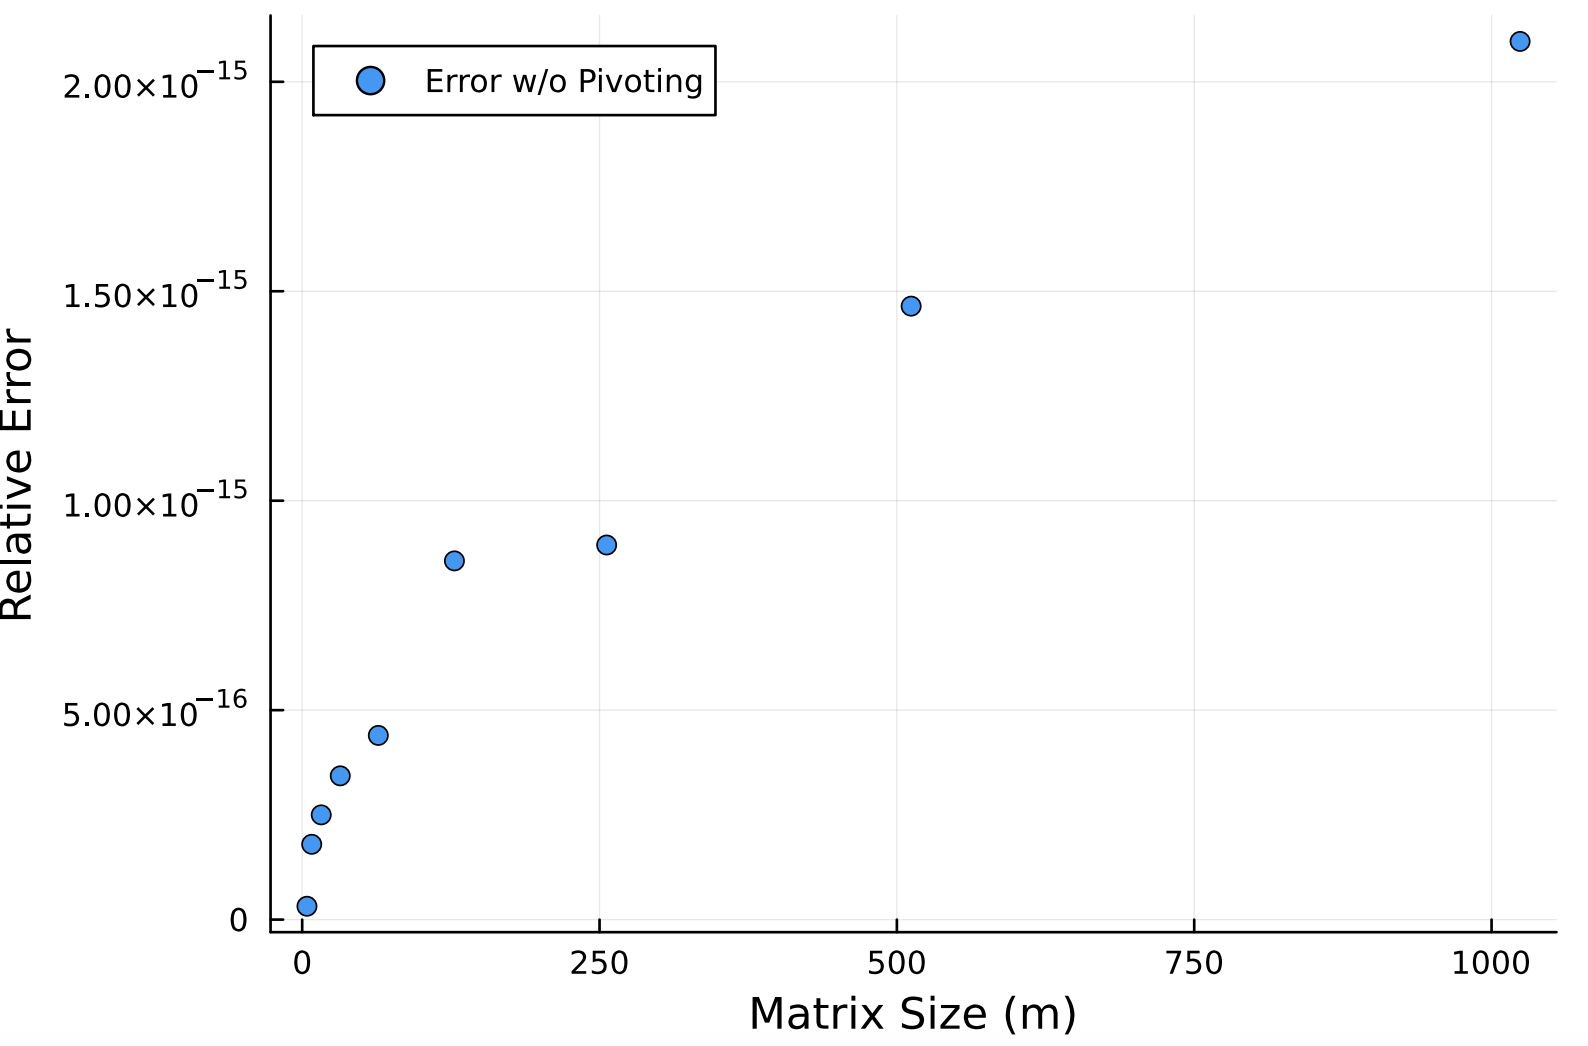
\includegraphics[width=0.75\linewidth]{Image 2-20-24 at 07.49.jpeg}
    \end{figure}

\begin{figure}[H]
    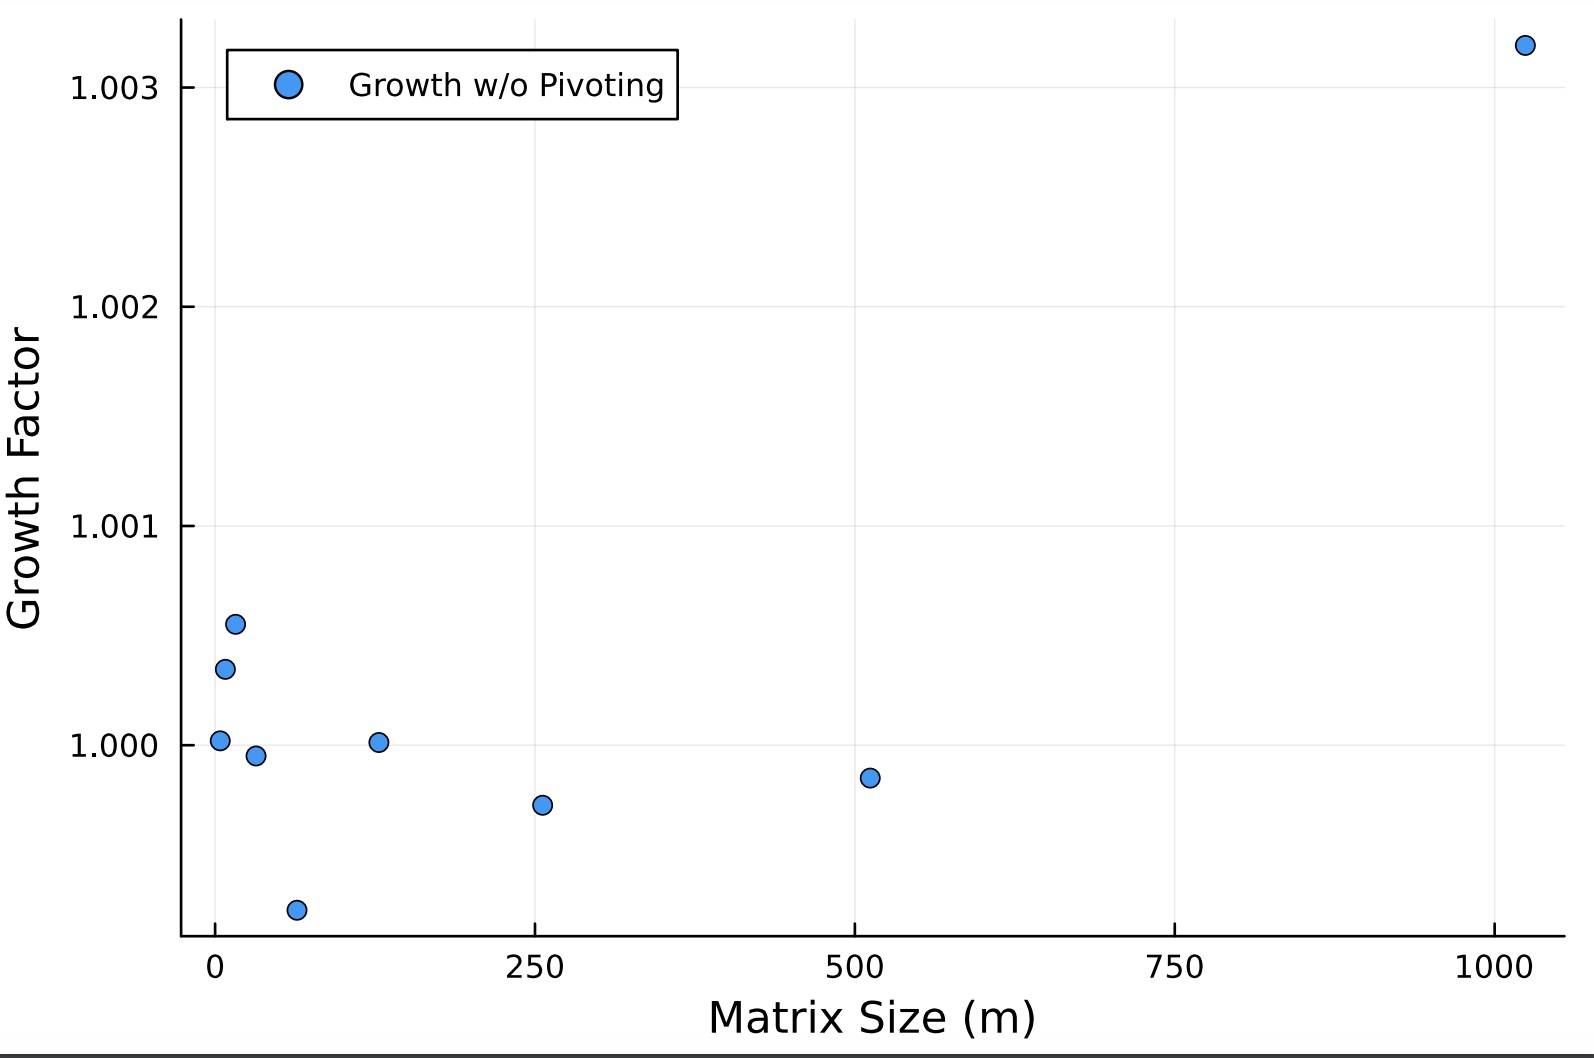
\includegraphics[width=0.75\linewidth]{Image 2-20-24 at 07.49 (1).jpeg}
    
    
\end{figure}
\subsection{(d)}
\begin{figure}[H]
    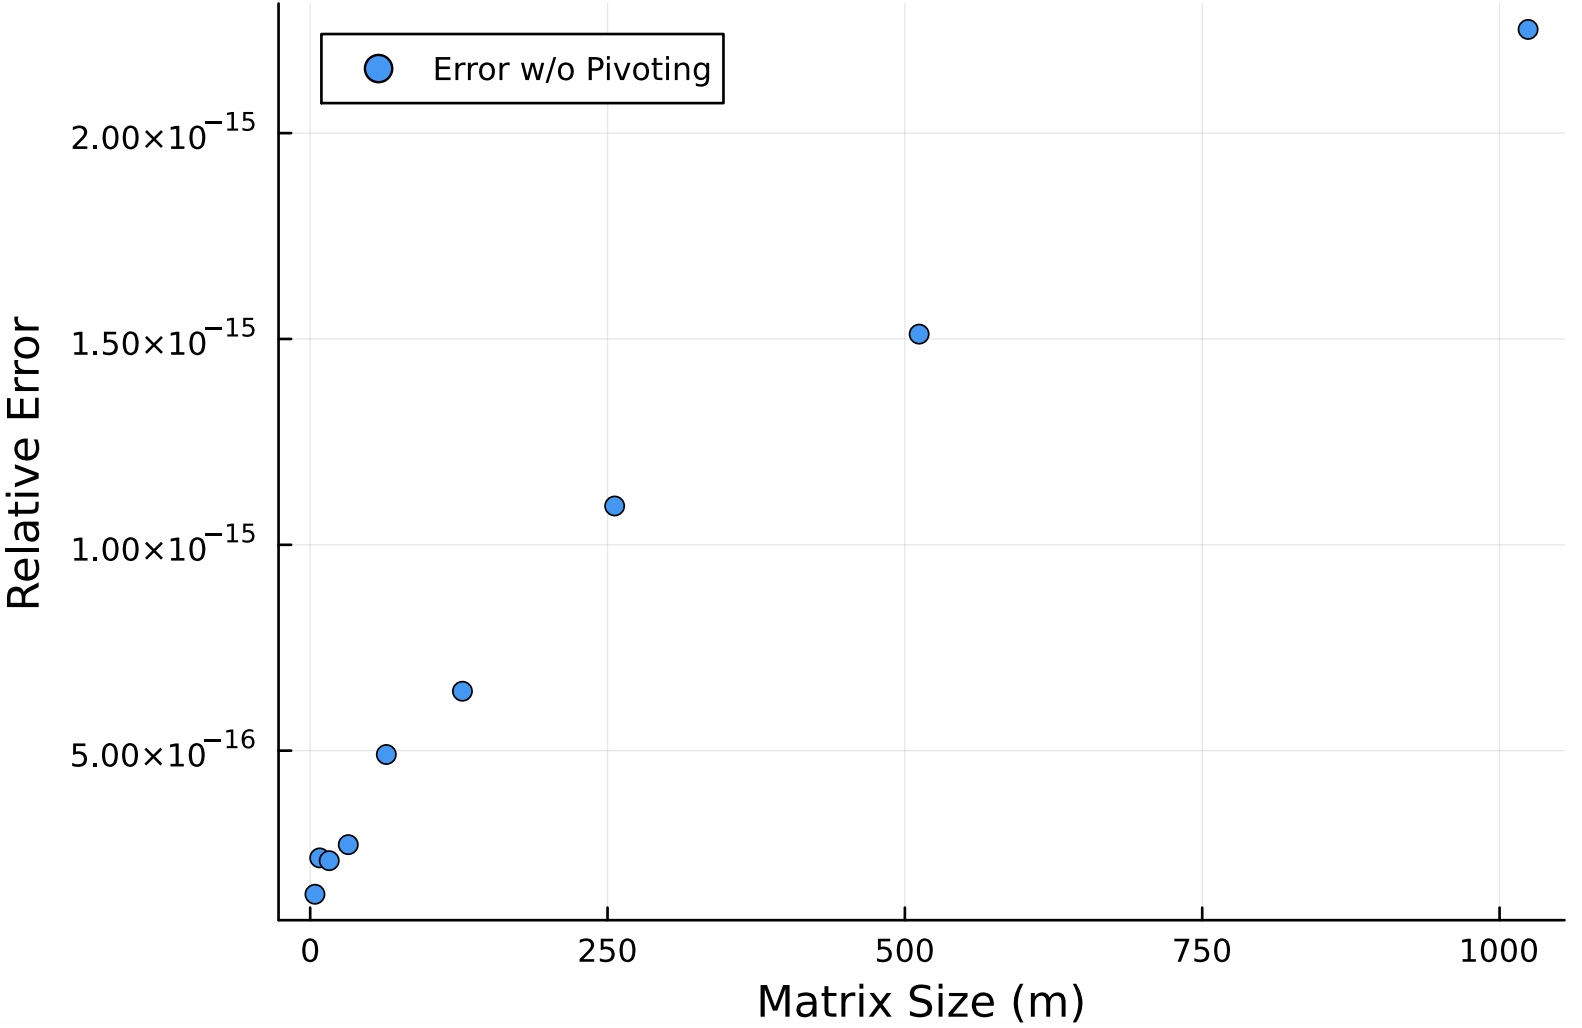
\includegraphics[width=0.75\linewidth]{Image 2-20-24 at 07.51.jpeg}
    
    
\end{figure}
\begin{figure}[H]
    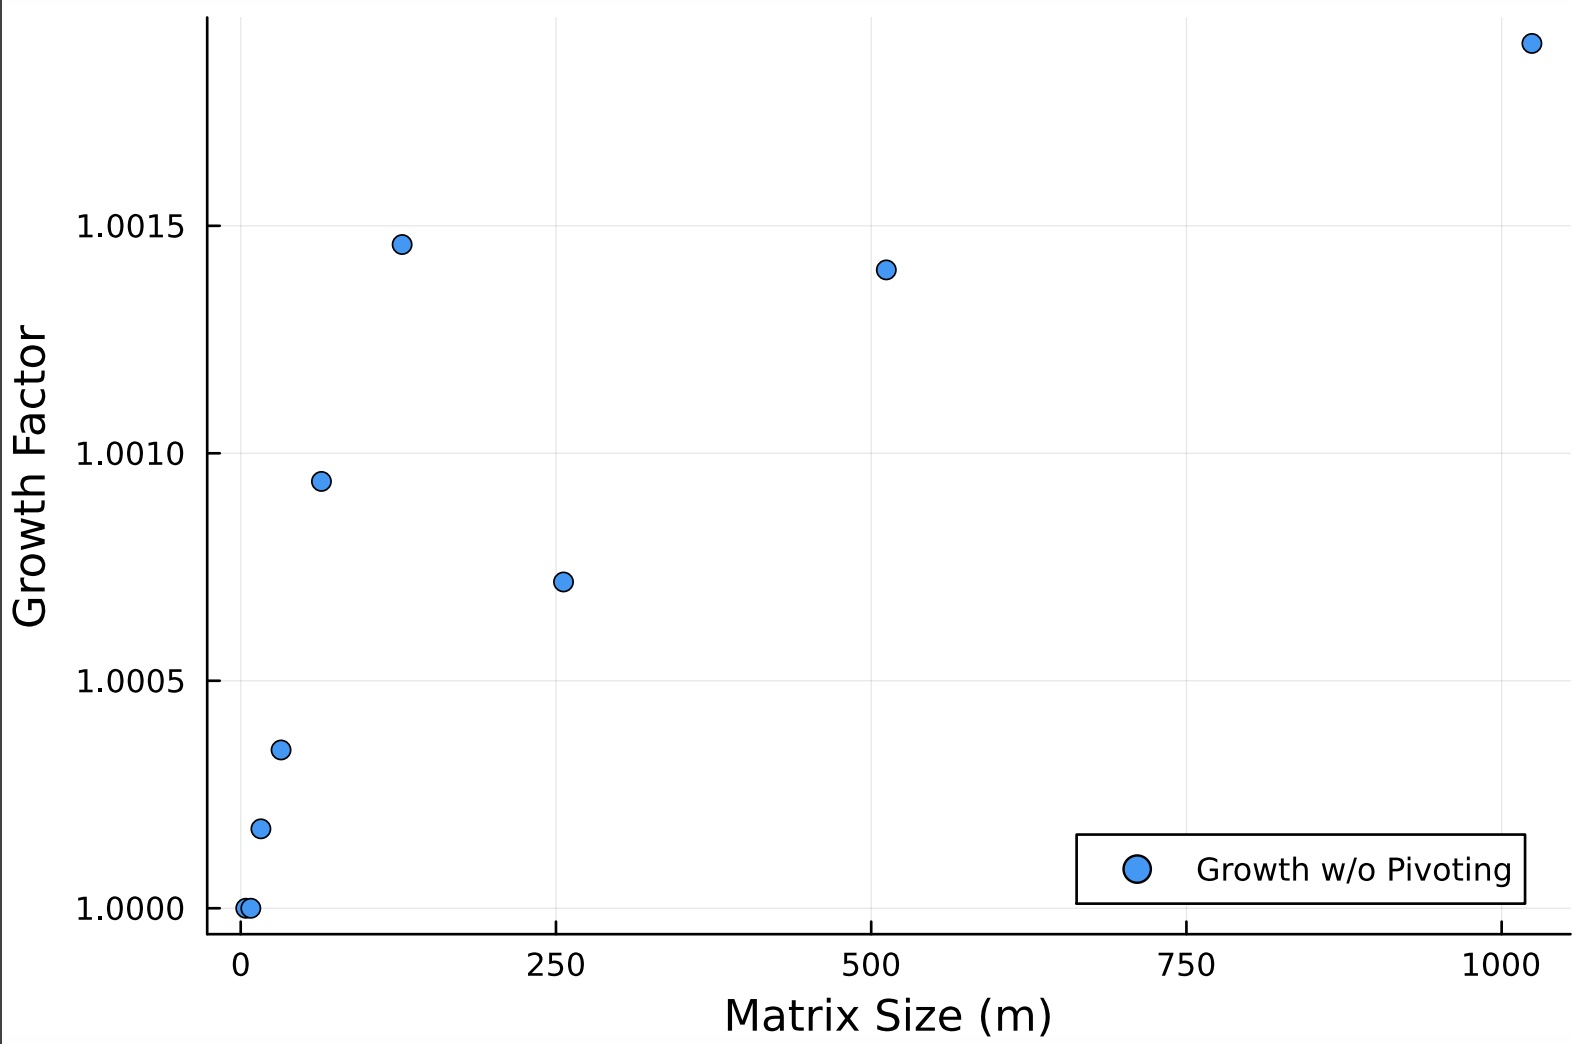
\includegraphics[width=0.75\linewidth]{Image 2-20-24 at 07.59.jpeg}
    
    
\end{figure}
\subsection{(e)}
\begin{figure}[H]
    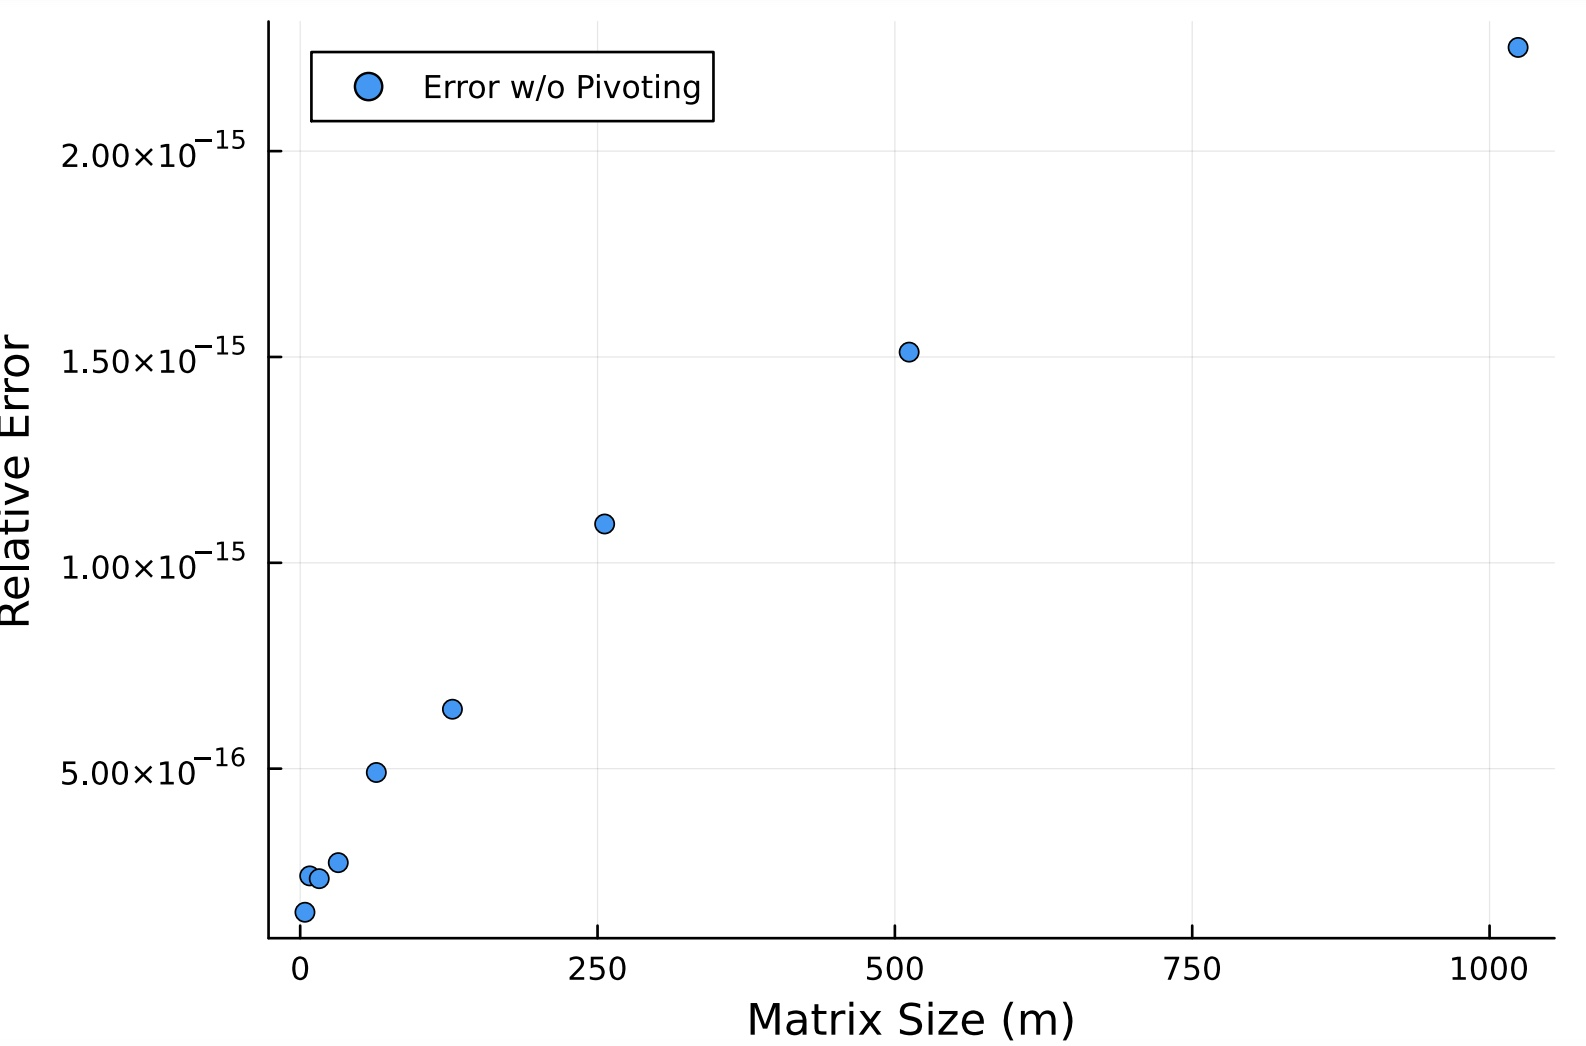
\includegraphics[width=0.75\linewidth]{Image 2-20-24 at 08.06.jpeg}
\end{figure}

\end{document}